\documentclass[a4paper,11pt]{scrreprt}

\usepackage[ngerman]{babel}
\usepackage[utf8]{inputenc}
\usepackage{amsthm}
\usepackage{enumerate}
\usepackage{mathtools}
\usepackage{amssymb}
\usepackage{stmaryrd}
\usepackage{listings}
\usepackage[dvipsnames]{xcolor}
\usepackage{hyperref}

\usepackage[headsepline]{scrlayer-scrpage}
\pagestyle{scrheadings}
\clearscrheadfoot
\ohead{Elisa Junghans\\Mirko Dransfeld}
\ihead{Wissenschaftliches Rechnen\\SS 19}
\chead{Praktikum MatLab\\Rubik's Cube}
\cfoot*{\pagemark}

\title{Rubik's Cube}
\subtitle{MatLab Praktikum\\Grundlagen des wissenschaftlichen Rechnens}
\author{Elisa Junghans (60186)\and Mirko Dransfeld (60653)}
\date{Sommersemester 2019}

\setcounter{secnumdepth}{4}

\hypersetup{
    unicode=true,
    colorlinks=true,
    linkcolor=BlueViolet,
    linktoc=all,
    citecolor=NavyBlue,
    filecolor=NavyBlue,
    urlcolor=NavyBlue,
    final=true
}

\lstset{ %
    basicstyle=\small\ttfamily,
    language=Matlab,
    showtabs=false,
    tabsize=2,
    captionpos=t,
    breaklines=true,
    extendedchars=true,
    showstringspaces=false,
    flexiblecolumns=true,
    numbers=left,
    numbersep=8pt,
    stepnumber=1,
    numberstyle=\color{Gray},
    keywordstyle=\color{Blue},
    commentstyle=\color{ForestGreen}
}

\newcommand{\codeimport}[4][0]{
  \lstinputlisting[firstnumber=#2,tabsize=4,framexleftmargin=\the\dimexpr -18pt * #1\relax,numbersep=\the\dimexpr \the\dimexpr -18pt * #1\relax + 8pt\relax,xleftmargin=\the\dimexpr -18pt * #1\relax, linerange={#2-#3}]{#4}
}

\newcommand{\coderef}[1]{
  \texttt{\nameref{#1}}
}
\newcommand{\codeinline}[1]{
  \lstinline!#1!
}
\newcommand{\codecustomref}[2]{
  \hyperref[#2]{\lstinline!#1!}
}


\newcommand{\chap}[2]{
  \chapter{#1}\label{#2}
}
\renewcommand{\sec}[2]{
  \section{#1}\label{#2}
}
\newcommand{\subsec}[2]{
  \subsection{#1}\label{#2}
}
\newcommand{\subsubsec}[2]{
  \subsubsection{#1}\label{#2}
}

%%
%%
%%
%%  Hallo Elisa :)
%%
%%
%%
%%  Überschriften sind: (absteigende Wichtigkeit)
%%  \chap{}{}       Kapitel
%%  \sec{}{}        sektion   (ist das ein wort?)
%%  \subsec{}{}     untersektion
%%  \subsubsec{}{}  unteruntersektion
%%
%%  alle funktionieren mit z.B. \chap{<Überschrift>}{<Labelname>}
%%  Die Labelnamen sind dafür um später auf die Funktion verweisen zu können, siehe \coderef
%%  Wichtig: Unterstriche in den Überschrifter escapen mit \_ !
%%
%%
%%
%%  wenn du Code aus einer Datei einbinden willst: \codeimport{<Anfang>}{<Ende>}{<Datei>}
%%  z.B.  \codeimport{44}{49}{RubiksCube}  fügt Zeilen 44-49 aus RubiksCube.m ein
%%
%%  wenn du eine bestimmte Funktion referenzieren willst: \coderef{<Labelname>}
%%  z.B.  \coderef{sec:figure}  macht daraus figure() mit einem Verweis zu \sec{figure()}{figure}. (es setzt den Funktionsnamen ein, so wie du ihn benannt hast)
%%
%%  wenn du einen kleinen inline-codeteil haben willst: \codeinline{<Text>}
%%  z.B.  \codeinline{figure(Option1, Wert1, ...)}  schreibt den <Text> als Code (inline)
%%
%%
%%
%%  Kannst dir ja das angucken was ich bisher geschrieben habe. Bei Problemen oder Feature-Wünschen -> Hey :)
%%
%%
%%

\begin{document}
  \maketitle
  \tableofcontents

  \chap{Aufbau des Programms}{aufbau}
    \sec{RubiksCube.m}{rubikscube}
      \subsec{Variablen}{variablen}
        \subsubsec{face\_colors}{facecolors}
          Dies ist ein zweidimensionales Array, dass die Farben der einzelnen Flächen\footnote{Im Folgenden bezeichnen 'Seite' die 6 Seiten eines Würfels und 'Fläche' die 9 Flächen auf jeder Seite.} des Würfels speichert. Dabei entsprechen die Zahlen 1--6 der Seite des Würfels, deren Farbe die Flächen haben. Die erste Koordinate ist die Seiten- und die Zweite die Flächennummer auf der jeweiligen Seite.

          \codeinline{face_colors(3,5)}wäre dementsprechend Fläche 5 auf Seite 3 (blau, unten rechts).
          \begin{figure}[!h]
            \centering
            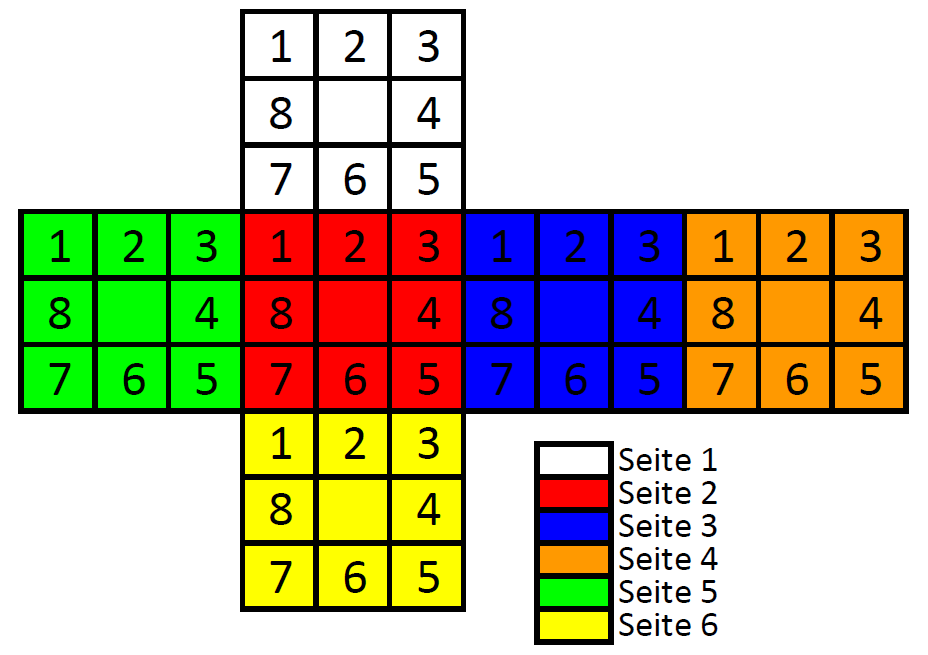
\includegraphics[width=0.5\columnwidth]{cubeMapCropped}
            \caption{Position der Flächen in\coderef{facecolors}}
          \end{figure}\newline
          Die Mittelflächen müssen hierbei nicht beachtet werden, da man ihre Position nicht durch Drehungen verändern kann. (siehe \autoref{grundlagen} \nameref{grundlagen})

        \subsubsec{rotation\_buttons}{rotationbuttons}
          Dies ist eine Liste an \coderef{uicontrol}-Elementen. Genauer sind dies die Knöpfe am linken Rand des UI, mit denen der Benutzer manuelle Drehungen des Würfels durchführen kann. Hierzu hat jeder Knopf eine UserData entspreched der Drehung, die dieser auslösen soll. Beim Klicken eines solchen Knopfes wird die Funktion\codeinline{manual_turn()}als \nameref{callback} aufgerufen, die dann mit Hilfe der UserData\coderef{turn}aufruft und somit den Würfel dreht.

      \subsec{Funktionen}{funktionen}
        \subsubsec{setup()}{setup}
          In dieser Funktion werden wichtige Variablen gesetzt, die während des Programmablaufs benötigt werden. Hierzu zählt unter anderem\codeinline{face_positions}für die Eckpunkte der Flächen. Außerdem wird\coderef{facecolors}mit den Standardwerten (gelöster Würfel) initialisiert.

        \subsubsec{main()}{main}
          Dies ist nach der\coderef{setup}Funktion die Zweite, die im Programmablauf aufgerufen wird. Zuerst wird mit\coderef{figure}die Figur erzeugt, in der der Würfel visualisiert wird. Danach folgen Aufrufe von\coderef{uisetup}und\coderef{generatepatchanduimenu}. Wenn anschließend die main-Funktion verlassen wird, ist das UI komplett erstellt und alle weiteren Funktionsaufrufe sind ein \nameref{callback}.

        \subsubsec{load\_presets()}{loadpresets}
          Diese Funktion interagiert mit der Datei\coderef{resources}und lädt sowohl die Farbdefinitionen für die Custom-Farbe, als auch die Presets in die Variablen\codeinline{color_dialog_colors}beziehungsweise\codeinline{cube_presets}. Die Datei wird mithlife der Funktion\codeinline{fgetl()}zeilenweise ohne newline-Zeichen ausgelesen. Dann werden mithlife von\codeinline{regexp()}die entsprechenden Teile extrahiert.

          Im folgenden Beispiel wird die erste Zeile zu Beginn in ein cell-Array aus je sechs hex-Zeichen aufgeteilt und dann mithilfe von \coderef{hex2rgb} in ein Array von RGB-Farben umgewandelt.
          \codeimport[3]{136}{137}{RubiksCube.m}

        \subsubsec{hex2rgb()}{hex2rgb}
          Diese Funktion wandelt ein cell-Array in ein Array von RGB-Farben um. Da RGB-Farben aus drei Komponenten bestehen, ist der Rückgabewert dieser Funktion ein zweidimensionales Array, bei dem man mit dem ersten Parameter die Farbe wählt und mit dem Zweiten auf die jeweiligen RGB-Komponenten zugreifen kann.

        \subsubsec{ui\_setup()}{uisetup}
          In dieser Funktion werden mithilfe von\coderef{uimenu}die Menüleiste angelegt und mit\coderef{uicontrol}die Elemente auf dem UI erzeugt, wie zum Beispiel die\coderef{rotationbuttons}. Außerdem werden die Achsen der Figur sowohl\codeinline{off}als auch\codeinline{equal}gesetzt und

          \coderef{generatecenterpieces}, \coderef{rotateview}, sowie \coderef{loadpresets} aufgerufen.

        \subsubsec{rotate\_view()}{rotateview}
          Diese Funktion rotiert die Figur in die Ausgangsposition mithilfe von: \codeimport[1]{377}{379}{RubiksCube.m}

        \subsubsec{generate\_centerpieces()}{generatecenterpieces}
          Mit\coderef{patch}werden die Mitten der Seiten erzeugt. Da diese durch die Drehungen nicht verändert werden können, sind diese nicht in\coderef{facecolors}enthalten.

        \subsubsec{solve\_cube()}{solvecube}
          Dies ist die Funktion, die als \nameref{callback} beim Klicken des solve-Buttons aufgerufen wird. Ziel dieser Funktion ist es, durch Aufruf von\coderef{generatesolution}, die Lösungsschritte zu erzeugen.

          Zu Beginn werden die UI-Elemente deaktiviert, um ein doppeltes Auslösen zu verhindern. Danach wird mit\codeinline{tabulate()}die absolute Häufigkeit der Farben in\coderef{facecolors}ermittelt. Wenn dies nicht acht für jede Farbe ergibt, muss es Farben doppelt geben und der Würfel ist nicht lösbar.
          \codeimport[2]{483}{486}{RubiksCube.m}
          Wenn dies nicht der Fall ist, wird\coderef{generatesolution}aufgerufen und der Rückgabewert in\codeinline{turn_list}gespeichert. Danach wir dieser ausgewertet:

          Ist\codeinline{turn_list}leer, ist der Würfel gelöst. Ist es -1, ist eine Lösung nicht möglich. Wenn beide Tests bestanden sind, sind demzufolge in\codeinline{turn_list}die Schritte zur Lösung gespeichert.

          Im Anschluss werden die deaktivierten UI-Elemente wieder freigegeben.

        \subsubsec{generate\_patch\_and\_ui\_menu()}{generatepatchanduimenu}
          Hier werden die Flächen und das zugehörige Kontextmenü generiert. Dazu wird zuerst das Kontextmenü für jede Fläche erzeugt und dann mit\codeinline{update_patches()}diese Flächen gezeichnet. Dies ist notwendig, da bei einem Klick auf ein Kontextmenü immer die Funktion\codeinline{change_color()}aufgerufen wird. Um nun unterscheiden zu können welche Fläche geändert werden soll, hat jedes Kontextmenü in seiner\codeinline{UserData}die Koordinaten der jeweiligen Fläche in\coderef{facecolors}, welcher es zugeordnet ist.

      \subsec{Callback}{callback}
        Ein Callback ist eine Funktion, die in Reaktion auf ein Geschehnis im Programmablauf aufgerufen wird. In unserem Fall sind diese Geschehnisse Interaktionen des Benutzers mit dem Programm. Nach der Erzeugung des UI führt das Programm keine weiteren Befehle aus, bis der Benutzer mit ihm interagiert. In den meisten Fällen ist dies ein Klick auf einen Knopf. MatLab bietet die Möglichkeit an UI-Elemente Callbacks als Parameter während der Erstellung anzuhängen. In unserem Fall haben wir dies dafür genutzt, um zum Beispiel das Lösen des Würfels nur zu beginnen, wenn der Benutzer auf den solve-Button klickt. Dies wurde realisiert, indem bei der Erstellung des Knopfes ein Funktionshandle übergeben wurde. \codeimport[2]{93}{93}{RubiksCube.m}

    \sec{turn.m}{turn}
      Diese Datei beinhaltet die Funktionen zum Drehen des Würfels. Dazu werden die Elemente von\codeinline{cube}je nach Drehung vertauscht. Diese Drehung wird durch \texttt{dir} bestimmt. Der Aufbau von\codeinline{cube}entspricht dem der\coderef{facecolors}. \texttt{dir} ist eine Zahl von 1--12. In einem\codeinline{switch}-Statement wird dann die jeweilige Rotation (siehe \autoref{grundlagen} \nameref{grundlagen}) ausgeführt.

    \sec{generate\_solution.m}{generatesolution}
      Am Anfang wird die Variable\coderef{facecolors}in eine lokale Variable kopiert und danach die Datei\coderef{f2lrecursive}aufgerufen. Sollte diese kein Ergebnis liefern oder abbrechen, so werden die ersten beiden Ebenen mit dem Lösungsalgorithmus für die \nameref{f2l} (\autoref{f2l}) gelöst. Danach wird die \nameref{oben} (\autoref{oben}) mit der Fridrich-Methode gelöst.

      Dabei ist jeder einzelne Schritt in einer eigenen Funktion umgesetzt. Sollte währenddessen ein nicht lösbarer Zustand festgestellt werden, wird die Variable\codeinline{turn_list}auf -1 gesetzt und die Funktion beendet. Andernfalls wird mit\codeinline{refresh_face_colors()}der lokale Zustand des Würfels für den nächsten Schritt aktualisiert.

      Wurde eine Lösung gefunden, wird sie in\codeinline{clean_up_output()}nach Möglichkeit verkürzt.

    \sec{f2l\_recursive.m}{f2lrecursive}
      Dies ist eine Umsetzung des \hyperref[recursive]{rekursiven Ansatzes}. Dabei wird die Anzahl der richtigen Flächen in der Funktion\codeinline{calc_fitness()}berechnet. Aufgrund des Verlaufs der Rekursion werden die Lösungsschritte in umgekehrter Reihenfolge ausgegeben.

    \sec{resources.txt}{resources}
      In der ersten Zeile werden, wenn festgelegt, die RGB-Farben für die Custom-Farboption in der Reihenfolge Oben-Vorne-Rechts-Hinten-Links-Unten definiert. Alle weiteren Zeilen beinhalten die Presets mit zugehörigem Namen. Bei Programmstart wird diese Datei in der Funktion\coderef{loadpresets}geladen.

  \chap{Lösungsalgorithmus}{algorithm}
    \sec{Grundlagen}{grundlagen}
      Die Algorithmen zum Lösen eines Zauberwürfels werden mit Buchstaben angegeben, um sie einfach notieren zu können.

      Dabei steht beispielsweise ein R dafür, dass die rechte Seite nach oben gedreht wird. Ebenso steht L für die linke, U für die obere, D für die untere, F für die vordere und B für die hintere Seite. Weitere Notationen sind für unsere Lösung irrelevant, da die Mitten nicht bewegt werden. Stehen die Buchstaben alleine, so werden sie, wenn man frontal auf die zu drehende Seite schaut, im Uhrzeigersinn gedreht. Steht hinter dem Buchstaben ein ', so werden sie in die entgegengesetzte Richtung gedreht. Folgt auf den Buchstaben eine 2 so wird die Bewegung zweimal ausgeführt.
      \begin{figure}[!h]
        \centering
        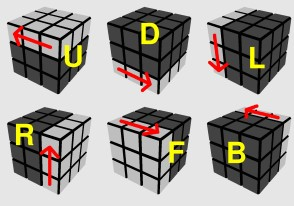
\includegraphics[width=0.5\columnwidth]{cubeRotations}
        \caption{Rotationen}
      \end{figure}

    \sec{untere und mittlere Ebene}{f2l}
      Da die ersten beiden Ebenen nicht wie gewöhnlich intuitiv gelöst werden können, müssen viele kleine Schritte gemacht werden, um zum Ziel zu gelangen.
      Daher werden zuerst die Kanten der untersten Ebene einzeln an ihre Position gebracht, indem sie nacheinander lokalisiert werden und dann je nach Position Algorithmen ausgeführt werden.

      Danach werden die Ecken der untersten Ebene an ihren Platz bewegt. Dies geschieht zuerst unabhängig von ihrer richtigen Position. Anschließend werden sie so getauscht, dass alle an ihrem Platz sind.
      Damit ist die unterste Ebene gelöst.

      Bei der zweiten Ebene müssen nur vier Kanten sortiert werden. Dies geschieht mit der Anfänger-Methode zum Lösen des Zauberwürfels. Dabei werden nacheinander die Kanten gesucht und an ihren Platz gedreht. Danach ist auch die zweite Ebene fertig.

    \sec{obere Ebene}{oben}
      Die oberste Ebene wird mittels der 2-Look Fridrich-Methode gelöst. Bei der eigentlichen Fridrich-Methode werden zuerst die Teile der letzten Seite orientiert und dann permutiert. Bei dieser Variante wird allerdings beides in zwei Schritten durchgeführt, wodurch weniger Algorithmen notwendig sind.
      Dabei werden zuerst die Kanten gekippt, sodass sie alle mit der gleichen Farbe nach oben zeigen.

      Danach werden die Ecken so gedreht, dass alle Flächen der oberen Seite die gleiche Farbe haben.
      Anschließend werden erst alle Ecken und dann alle Kanten permutiert. Damit ist der Würfel gelöst.

    \sec{rekursiver Ansatz}{recursive}
      Ein anderer Ansatz wäre jede mögliche Bewegung für den nächsten Zug auszuprobieren und für jeden die Flächen zu zählen, die an der richtigen Position sind. Dann werden rekursiv alle Möglichkeiten durchgetesetet, die eine Verbesserung darstellen. Sollte keine der Möglichkeiten die Lösung des Zauberwürfels voranbringen, so wird abgebrochen.

      Sollte der Würfel gelöst sein, so wird ebenfalls abgebrochen und keine weitere Drehung durchgeführt. Wenn sich die Anzahl mit jeder Drehung verbessern soll, so wird dies schnell zu einem Abbruch führen. Das liegt daran, dass die für den nächsten Zug beste Drehung nicht unbedingt die ist, welche auch zum optimalen Lösungsweg oder überhaupt zu einer Lösung führt.

  \chap{Besondere MatLab-Funktionen}{matlab}
    \sec{figure()}{figure}
      Dieser Befehl erzeugt eine neue Figur. Die Eigenschaften werden ähnlich einer\codeinline{struct}in der Form\codeinline{figure('Parameter1', 'Wert1', 'Parameter2', 'Wert2', ...)}übergeben.

    \sec{patch()}{patch}
      Mit\coderef{patch}können Vielecke in eine Figur gezeichnet werden. Hierzu werden die Eckpunkte als Vektoren übergeben, in unserem Fall in der Form\codecustomref{patch(X, Y, Z)}{patch}wobei\codeinline{X, Y, Z}jeweils die gleiche Länge haben.

    \sec{uicontrol()}{uicontrol}
      Dieser Befehl erzeugt UI-Elemente. Ähnlich wie\coderef{figure}werden die Parameter wie die einer\codeinline{struct}übergeben. Mit dem Parameter\codeinline{'Style'}kann hierbei die Art des UI-Elementes bestimmt werden. Dies können zum Beispiel\codeinline{'pushbutton'},\codeinline{'text'},\codeinline{'checkbox'}oder\codeinline{'slider'}sein.

    \sec{uimenu()}{uimenu}
      Hiermit können unter anderem Kontextmenüeinträge oder auch Elemente der MenuBar erzeugt werden. Wenn als erster Parameter ein weiteres UIMenu üebergeben wird, wird das neue als Untermenü des Vorigen erstellt. Die anderen Parameter sind wie\coderef{figure}oder\coderef{uicontrol}im Stil einer\codeinline{struct}anzugeben.

    \sec{dialog()}{dialog}
      Mit diesem Befehl können Dialogfelder erzeugt werden. Wiederum können Parameter wie\codeinline{'Name'}ähnlich wie bei einer\codeinline{struct}übergeben werden. Je nach Anwendungszweck können auch spezialisterte Alternativen verwendet werden, wie zum Beispiel\codeinline{uisetcolor()}für einen Farbauswahldialog.

\end{document}
